\section{Experiments}
\label{sec:experiments}

Our experiments were intended to study MAC's and S-MAC's generalization as well as transfer learning abilities in different settings. We used CLEVR and CoGenT to address these different aspects.
The first experiment studied the training time and the capability of the models to generalize on the same type of dataset that it was trained on. This was used mainly as a baseline for the further experiments that were intended to study how well the transfer learning performed in comparison to the baseline results.
The second experiment studied the capability of the models to succeed in doing transfer learning from domain A to domain B when trained on different combinations of the respective domains. The third experiment was intended to see whether the performance improves if the model could be further trained on a small subset of the dataset from domain B.
\tableref{results} presents the most important results, focusing on S-MAC in particular; see Appendix~\ref{sec:full_comparison} for the entire set.

For all experiments, the initial training procedure is as follows: we train the given model  for 20 epochs on 90\% of the training sets of CLEVR \& CoGenT separately. We keep the remaining 10\% for validating the model at every epoch, and use the original validation sets as test sets.
%given that the ground truth labels for the true test sets are not available.

Our implementation of both MAC models used PyTorch (v0.4.0)~\cite{paszke2017automatic}. We relied on the MI-Prometheus~\cite{kornuta2018accelerating} framework that enables fast experimentation of the cross product of models and datasets\footnote{To reproduce the presented research please follow:  \url{https://github.com/IBM/mi-prometheus/}}.
We used NVIDIA's GeForce GTX TITAN X GPUs. We followed the implementation details indicated in the supplemental material (Sec. A) of the original paper~\cite{hudson2018compositional}, to ensure a faithful comparison.

\subsection{Transfer Learning}
\label{sec:transfer_learning}

\begin{table}[t]
	\caption{CLEVR \& CoGenT accuracies for the MAC \& S-MAC models. The [Training] column indicates wall times and final accuracies on the training set. For fine-tuning, we use 30k samples of the test set, and kept the remainder for testing. The [Fine-tuning] column reports the used sub-set (30k samples) and the final accuracies on this sub-set during training. The [Test] column reports the used set and the obtained test accuracies. If no fine-tuning was done, the whole indicated set was used for testing.}
	\centering
	\begin{tabular}{cccccCcCC}
		\toprule
		\multirow{2}{*}{Model} & \multicolumn{3}{c}{Training} &  \multicolumn{2}{c}{Fine-tuning} & \multicolumn{2}{c}{Test} & \multirow{2}{*}{Row} \\
		\cmidrule{2-4} \cmidrule{5-6} \cmidrule{7-8} 
		& Dataset                & Time [h:m] & Acc [\%]          & Dataset & Acc [\%]  & Dataset & Acc [\%] & \\
		\midrule
		MAC & CLEVR  & 30:52  & 96.70 & --   & --  & CLEVR    & 96.17         & (a) \\
		\cmidrule{1-8}
		\cmidrule{1-8}
				
		 \multirow{13}{*}{S-MAC} & CLEVR  & 28:30  & 95.82 & --   & --  & CLEVR    & 95.29         & (b)  \\
		 \cmidrule{2-4} \cmidrule{5-6} \cmidrule{7-8} 
		
		& CoGenT-A  & 28:33   & 96.09 &  --  &  --  & CoGenT-A & 95.91        & (c)  \\
		\cmidrule{2-4} \cmidrule{5-6} \cmidrule{7-8} 
		
		
		& \multirow{2}{*}{CLEVR}  & \multirow{2}{*}{28:30}  & \multirow{2}{*}{95.82} & \multirow{2}{*}{--}   & \multirow{2}{*}{--}  &   CoGenT-A    &  95.47  & (d) \\
		\cmidrule{7-8} 
		&                        &   &              &     &                               & CoGenT-B   &  95.58  & (e)\\		
				
		\cmidrule{2-4} \cmidrule{5-6} \cmidrule{7-8} 
		& \multirow{4}{*}{CoGenT-A}   & \multirow{4}{*}{28:33}   & \multirow{4}{*}{96.09}  &  \multirow{1}{*}{--}  &  \multirow{1}{*}{--}   & CogenT-B & 78.71        & (f)  \\
		\cmidrule{5-6} \cmidrule{7-8} 
		&                             &                                         &    &   \multirow{2}{*}{CoGenT-B}         &       \multirow{2}{*}{96.85}          & CoGenT-A &  91.24        & (g) \\
		\cmidrule{7-8} 
		&                             &                                         &       &         &                & CoGenT-B &    94.55     & (h)  \\

		\cmidrule{2-4} \cmidrule{5-6} \cmidrule{7-8} 
& \multirow{2}{*}{CLEVR}  & \multirow{2}{*}{28:30}  & \multirow{2}{*}{95.82} &   \multirow{2}{*}{CoGenT-B}         &       \multirow{2}{*}{97.67}          & CoGenT-A &  92.11       & (i) \\
\cmidrule{7-8} 
&                             &                                         &       &         &                & CoGenT-B &    92.95    & (j)  \\  		


		\bottomrule
	\end{tabular}
	\label{results}
\end{table}

For the CLEVR dataset, the training wall time of MAC (row a) is consistent with what is reported in the original paper (roughly 30h of training for 20 epochs).
S-MAC trains faster, showing a decrease of 10.5\% in wall time (row b), due to the reductions in the 
number of parameters as shown earlier.
This was consistently observed across the other experiments as well.

Turning to the generalization performance (row a),  MAC on CLEVR yields an accuracy of 96.17\%, which is 
taken as a reference experiment. S-MAC reaches an accuracy of 95.29\% on CLEVR (row b), indicating that 
the simplifications did not hinder its generalization capability.
Similar performance was observed for generalization on CoGenT-A (row c).

Before fine-tuning, we wanted to estimate the best upper bounds on accuracy that we could possibly get by doing transfer learning.
As both CoGenT datasets contain complementary subsets of colors/shapes  combinations present in CLEVR, 
we evaluated CLEVR-trained models on the CoGenT datasets.
Even though the CoGenT datasets were generated using more restricted parameters, the models obtained nearly equal accuracy (rows d-e).

Evaluating S-MAC on CoGenT shows that, similar to~\cite{johnson2017inferring, mascharka2018transparency}, the score is worse on CoGenT-B (zero-shot learning, row f) than CoGenT-A after training on CoGenT-A data only (generalization, row c).

Following \cite{johnson2017inferring, perez2017film}), we then fine-tune S-MAC using 3k images and 30k questions from the CoGenT-B data (for 10 epochs), and re-evaluate it on both conditions. This enables much higher accuracy on CoGenT-B, of at least a 15 points increase (row h). Performance on CoGenT-A is slightly worse, dropping by 4 points (row g). This seems to indicate that S-MAC is able to learn new combinations of shape \& color without forgetting the ones it learned during the initial training. 

To study the pitfalls of fine-tuning, we conducted a final set of experiments, where we fine-tuned a CLEVR-trained S-MAC model on CoGenT-B for 10 epochs, as before. Surprisingly, this operation handicapped the generalization of the model not only on CoGenT-A (row i), but also on CoGenT-B (row j, a 3 point drop compared to row e). This highlights the delicate nature of fine-tuning, with respect to the correlation between the datasets. This warrants further investigations.


\subsection{Illustration of failures of MAC on CLEVR}
\label{sec:failures}

Following the evaluation of MAC on CoGenT-B, we built a tool which helped us visualizing the attention of the model over the question words and the image, and thus provide insight on some cases of failure.

\fig{fig:fail_mac_shape} presents a question where the model is asked about the shape of the leftmost gray cylinder. The model correctly finds it, as we can see from its visual attention map, and appears to refer to it using its color (\textit{gray}), as we can see from the attention of the question words. Yet, it defaults to predicting the shape as \textit{cube}, because it never saw gray cylinders during training, but instead saw gray cubes.

\fig{fig:fail_mac_color} presents a similar case, where the model is questioned about the color of the green cube at the back. MAC misses that object, and instead focuses on the nearby gray cylinder. We can hypothesize that MAC missed the green cube as it did not see this combination during training, and thus defaulted to a combination that it knows.


\begin{figure}[htbp]
	\centering
	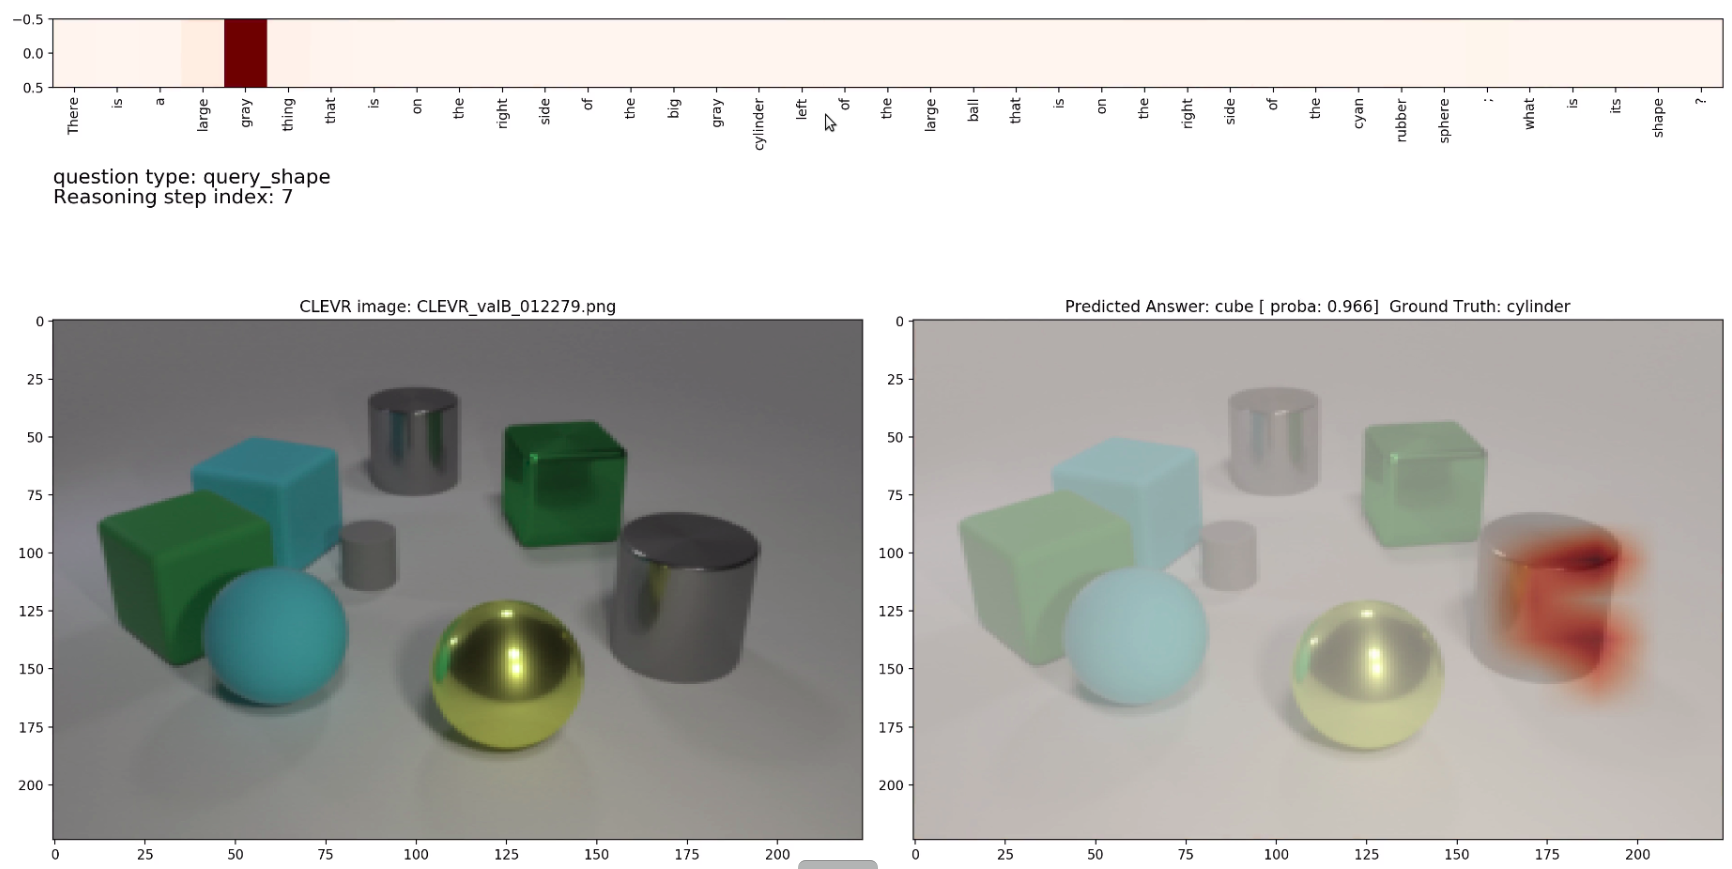
\includegraphics[width=\textwidth]{../img/fail_mac_cogent_b_shape.png}
	\caption{The question reads as: \textit{There is a large gray thing that is on the right side of the big gray cylinder left of the large ball that is on the right side if the cyan rubber sphere; what is its shape?}}
	\label{fig:fail_mac_shape}
\end{figure}

\begin{figure}[htbp]
	\centering
	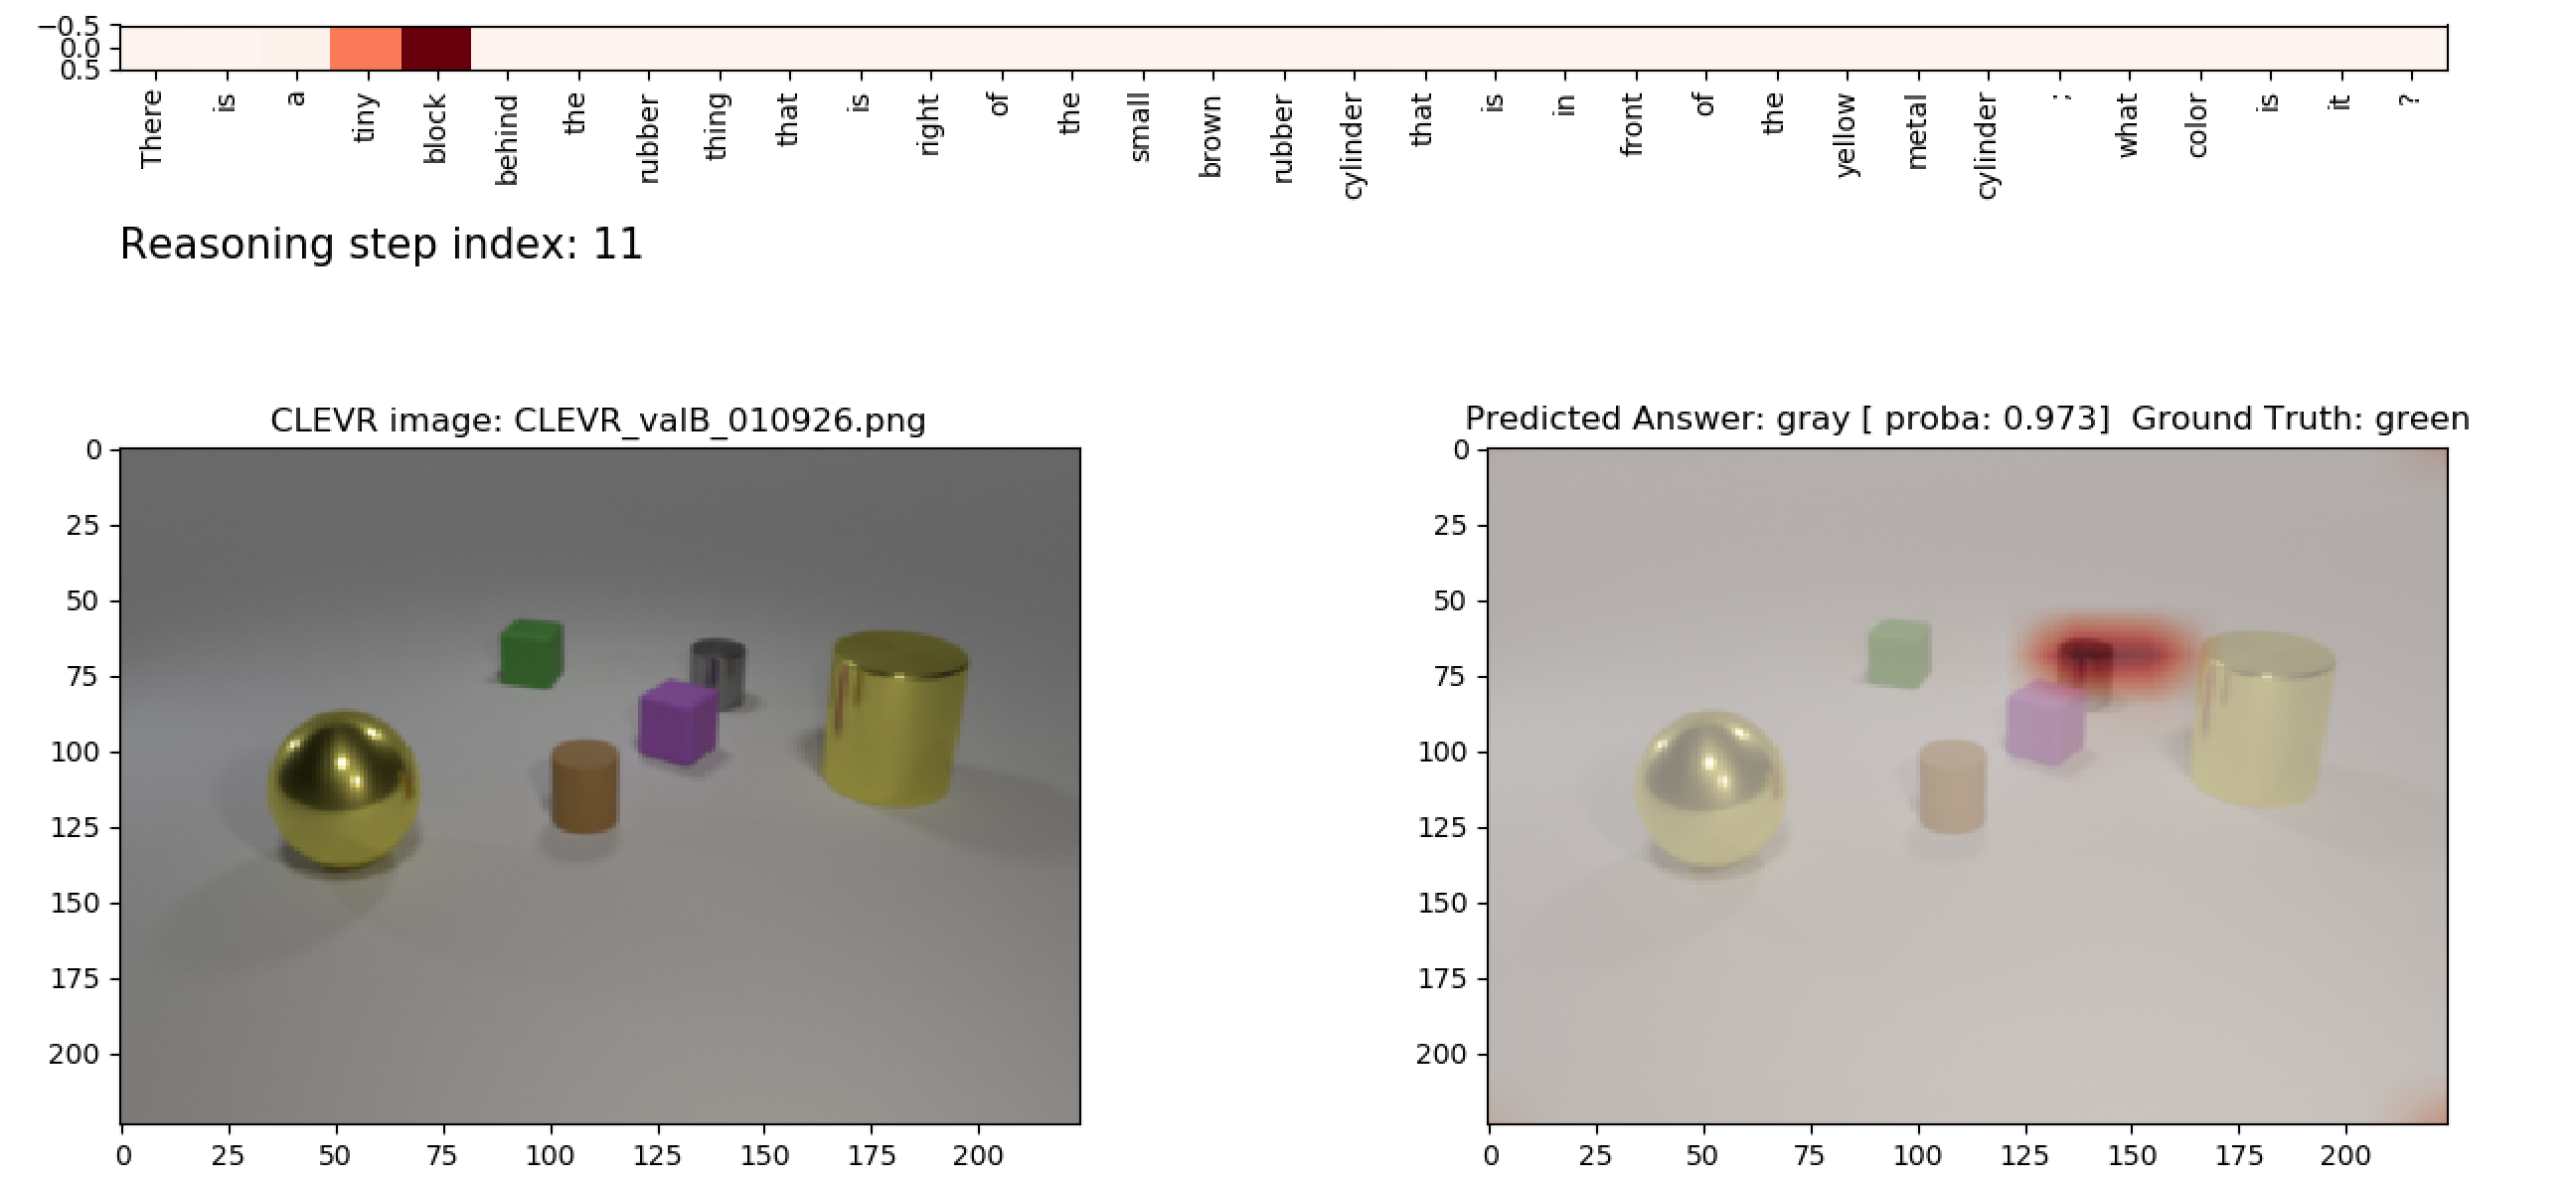
\includegraphics[width=\textwidth]{../img/fail_mac_cogent_b_color.png}
	\caption{The question reads as: \textit{There is a tiny block behind the rubber thing that is right if the small brown rubber cylinder that is in front of the yellow metal cylinder; what color is it?}}
	\label{fig:fail_mac_color}
\end{figure}

Those examples indicate that MAC did not correctly separate the concept of shape from the concept of color, but have a better understanding of the colors (as it found the object of interest in \fig{fig:fail_mac_shape} by its color). This could come from that fact that the shape \textit{sphere} is associated with all possible colors in the dataset. 
